\documentclass[12pt,a4paper]{article}

% ─── Page Layout ───────────────────────────────────────────────────────────────
\usepackage[a4paper, margin=0.8in, headheight=14pt]{geometry}

% ─── Fonts (XeLaTeX) ───────────────────────────────────────────────────────────
\usepackage{fontspec}
\usepackage{unicode-math}
\setmainfont{TeX Gyre Pagella}
\setmonofont[Scale=0.88]{TeX Gyre Cursor}
\setmathfont{Latin Modern Math}

% ─── Packages ──────────────────────────────────────────────────────────────────
\usepackage{xcolor}
\usepackage{colortbl}
\usepackage{titlesec}
\usepackage{enumitem}
\usepackage{tabularx}
\usepackage{booktabs}
\usepackage{array}
\usepackage{amsmath}
\usepackage{tikz}
\usetikzlibrary{shapes.geometric, arrows.meta, positioning, calc, fit, decorations.pathreplacing}
\usepackage{tcolorbox}
\tcbuselibrary{skins, breakable}
\usepackage{hyperref}
\usepackage{fancyhdr}
\usepackage{graphicx}
\usepackage{microtype}
\hyphenpenalty=10000
\exhyphenpenalty=10000
\sloppy
\usepackage{caption}
\usepackage{setspace}
\usepackage{multirow}
\usepackage{tocloft}

% ─── Q&A helper ────────────────────────────────────────────────────────────────
\newcommand{\Q}[1]{\textbf{#1}\par\noindent\ignorespaces}

% ─── Colour Palette ────────────────────────────────────────────────────────────
\definecolor{myred}{RGB}{196,30,58}
\definecolor{mydark}{RGB}{30,30,50}
\definecolor{mygreen}{RGB}{14,120,80}
\definecolor{myteal}{RGB}{0,130,140}
\definecolor{myamber}{RGB}{180,100,0}
\definecolor{mypurple}{RGB}{100,30,160}
\definecolor{mygray}{RGB}{246,247,249}
\definecolor{mgframe}{RGB}{180,185,200}
\definecolor{watermark}{RGB}{145,150,170}
\definecolor{hdrred}{RGB}{250,232,235}
\definecolor{hdrgreen}{RGB}{220,244,233}
\definecolor{hdrteal}{RGB}{220,242,244}
\definecolor{hdramber}{RGB}{253,242,215}
\definecolor{hdrpurple}{RGB}{238,228,255}
\definecolor{hdrgray}{RGB}{238,240,245}
\definecolor{rowalt}{RGB}{250,251,253}

% ─── Section Formatting ────────────────────────────────────────────────────────
\titleformat{\section}
  {\large\bfseries\color{myred}}{\thesection.}{0.5em}{}
  [\vspace{1pt}{\color{myred}\rule{\linewidth}{0.8pt}}]
\titleformat{\subsection}
  {\normalsize\bfseries\color{myteal}}{\thesubsection}{0.5em}{}
\titlespacing*{\section}{0pt}{18pt}{7pt}
\titlespacing*{\subsection}{0pt}{11pt}{4pt}

% ─── Paragraph ─────────────────────────────────────────────────────────────────
\setlength{\parindent}{0pt}
\setlength{\parskip}{4pt}

% ─── TOC Styling ───────────────────────────────────────────────────────────────
\renewcommand{\cfttoctitlefont}{\large\bfseries\color{myred}}
\renewcommand{\cftaftertoctitle}{\par\noindent{\color{myred}\rule{\linewidth}{0.8pt}}}
\setlength{\cftbeforetoctitleskip}{0pt}
\setlength{\cftaftertoctitleskip}{6pt}
\renewcommand{\cftsecfont}{\normalsize\bfseries\color{mydark}}
\renewcommand{\cftsecpagefont}{\normalsize\bfseries\color{mydark}}
\renewcommand{\cftsecleader}{\cftdotfill{\cftdotsep}}
\setlength{\cftbeforesecskip}{7pt}
\renewcommand{\cftsubsecfont}{\small\color{mydark}}
\renewcommand{\cftsubsecpagefont}{\small\color{mydark}}
\setlength{\cftbeforesubsecskip}{3pt}
\setlength{\cftsubsecindent}{1.4em}

% ─── Table helpers ─────────────────────────────────────────────────────────────
\renewcommand{\arraystretch}{1.45}
\setlength{\tabcolsep}{6pt}
\arrayrulecolor{mydark}
\newcolumntype{B}[1]{>{\small\bfseries\raggedright\arraybackslash}m{#1}}
\newcolumntype{Y}{>{\small\raggedright\arraybackslash}X}
\renewcommand{\tabularxcolumn}[1]{m{#1}}

% ─── Header / Footer ───────────────────────────────────────────────────────────
\pagestyle{fancy}
\fancyhf{}
\fancyhead[L]{\small\color{myred}\textbf{HS-HU701}\;\color{mydark}--- Principles of Management}
\fancyhead[R]{\small\color{myteal}\textbf{Module 4 Notes}}
\fancyfoot[C]{\small\color{mydark}\thepage}
\fancyfoot[R]{\small\color{watermark}\textit{\copyright\ Biraj}}
\renewcommand{\headrulewidth}{0.5pt}
\renewcommand{\footrulewidth}{0.3pt}

% ─── Hyperref ──────────────────────────────────────────────────────────────────
\hypersetup{
  colorlinks=true, linkcolor=myteal, urlcolor=myteal,
  pdfauthor={Biraj Sarkar},
  pdftitle={HS-HU701 --- Module 4 Notes}
}

% ─── tcolorbox styles ──────────────────────────────────────────────────────────
\tcbset{
  tikzbox/.style={
    colback=mygray, colframe=mgframe, boxrule=0.6pt, arc=4pt,
    left=8pt, right=8pt, top=6pt, bottom=6pt,
    colbacktitle=mgframe, coltitle=mydark,
    fonttitle=\small\bfseries
  },
  defbox/.style={
    colback=hdrgreen, colframe=mygreen, boxrule=0.8pt, arc=4pt,
    left=9pt, right=9pt, top=6pt, bottom=6pt,
    colbacktitle=mygreen, coltitle=white,
    fonttitle=\small\bfseries
  },
  formulabox/.style={
    colback=hdrteal, colframe=myteal, boxrule=0.8pt, arc=4pt,
    left=9pt, right=9pt, top=7pt, bottom=7pt,
    colbacktitle=myteal, coltitle=white,
    fonttitle=\small\bfseries
  },
  examplebox/.style={
    colback=hdramber, colframe=myamber, boxrule=0.8pt, arc=4pt,
    left=9pt, right=9pt, top=6pt, bottom=6pt,
    colbacktitle=myamber, coltitle=white,
    fonttitle=\small\bfseries
  },
  masonbox/.style={
    colback=hdrpurple, colframe=mypurple, boxrule=0.8pt, arc=4pt,
    left=9pt, right=9pt, top=6pt, bottom=6pt,
    colbacktitle=mypurple, coltitle=white,
    fonttitle=\small\bfseries
  },
  exambox/.style={
    colback=hdrpurple, colframe=mypurple, boxrule=1pt, arc=5pt,
    left=10pt, right=10pt, top=8pt, bottom=8pt,
    colbacktitle=mypurple, coltitle=white,
    fonttitle=\bfseries,
    breakable, title after break={\textbf{Frequently Asked / Viva Questions (contd.)}}}
}
\tcbset{breakable}

% ─── TikZ styles ───────────────────────────────────────────────────────────────
\tikzset{
  block/.style={rectangle, draw=myteal, fill=hdrteal,
    text width=2.4cm, align=center, minimum height=0.95cm,
    font=\small, rounded corners=3pt, line width=0.7pt},
  redblock/.style={rectangle, draw=myred, fill=hdrred,
    text width=2.4cm, align=center, minimum height=0.95cm,
    font=\small, rounded corners=3pt, line width=0.7pt},
  netnode/.style={rectangle, draw=myteal, fill=hdrteal,
    text width=1.5cm, align=center, minimum height=0.8cm,
    font=\small, rounded corners=3pt, line width=0.7pt},
  sumjunc/.style={circle, draw=myamber, fill=hdramber,
    minimum size=0.62cm, font=\small, line width=0.8pt},
  snode/.style={circle, draw=mypurple, fill=hdrpurple,
    minimum size=0.55cm, font=\footnotesize, line width=0.7pt},
  arrow/.style={-Stealth, thick, color=mydark},
  redarrow/.style={-Stealth, thick, color=myred},
  line/.style={thick, color=mydark}
}

% ═══════════════════════════════════════════════════════════════════════════════
\begin{document}
% ═══════════════════════════════════════════════════════════════════════════════

\begin{center}
  {\LARGE\bfseries\color{myred} HS-HU701 --- Principles of Management}\\[5pt]
  {\normalsize\color{mydark} Semester VII \quad$\bullet$\quad 2L:0T:0P \quad$\bullet$\quad 2 Credits}\\[3pt]
  {\normalsize\color{myteal}\textbf{Module 4 Exam Notes}}\\[3pt]
  {\small\color{mydark} CGEC \;$|$\; B.Tech ECE (2023--27) \;$|$\; \textit{Biraj Sarkar}}
\end{center}
\vspace{2pt}
\noindent{\color{myred}\rule{\linewidth}{1.5pt}}
\vspace{2pt}

\hypersetup{linkcolor=mydark}
\tableofcontents
\hypersetup{linkcolor=myteal}
\newpage

% ===============================================================================
\section{Customer Management}
% ===============================================================================

\begin{tcolorbox}[defbox, title={\textbf{Customer Management --- Overview}}]
\textbf{Customer Management} encompasses all strategies and activities through which an organisation attracts, retains, and grows its customer base. It includes market planning, research, the marketing mix, advertising, and brand management --- all directed toward satisfying customer needs profitably.
\end{tcolorbox}

\subsection{Market Planning and Research}

\begin{tcolorbox}[defbox, title={\textbf{Market Planning and Marketing Research}}]
\textbf{Market Planning} is the process of setting marketing objectives and devising strategies and tactics to achieve them. It involves analysing the market environment, identifying target segments, and allocating resources.
\par\vspace{3pt}
\textbf{Marketing Research} is the systematic gathering, recording, and analysis of data about problems relating to the marketing of goods and services. It bridges the gap between the organisation and its customers.
\end{tcolorbox}

\textbf{Steps in the Marketing Research Process:}
\begin{enumerate}[label=\textbf{\arabic*.}, leftmargin=*, itemsep=3pt, topsep=2pt]
  \item \textbf{Define the Problem and Research Objectives:} Clearly state what information is needed.
  \item \textbf{Develop the Research Plan:} Choose data sources (primary/secondary), research methods (survey, observation, experiment), and sampling plan.
  \item \textbf{Collect Information:} Gather primary data (questionnaires, interviews, focus groups) or secondary data (reports, databases).
  \item \textbf{Analyse the Information:} Tabulate, cross-tabulate, and apply statistical techniques.
  \item \textbf{Present the Findings:} Report actionable conclusions to management.
  \item \textbf{Make the Decision:} Use findings to guide marketing strategy.
\end{enumerate}

\subsection{The Marketing Mix --- 4Ps}

\begin{tcolorbox}[defbox, title={\textbf{Marketing Mix (4Ps)}}]
The \textbf{Marketing Mix} is the set of controllable, tactical marketing tools that the firm blends to produce the response it wants in the target market. The four Ps are: \textbf{Product, Price, Place (Distribution), and Promotion}.
\end{tcolorbox}

\begin{tcolorbox}[tikzbox, title={The 4Ps of the Marketing Mix}]
\centering
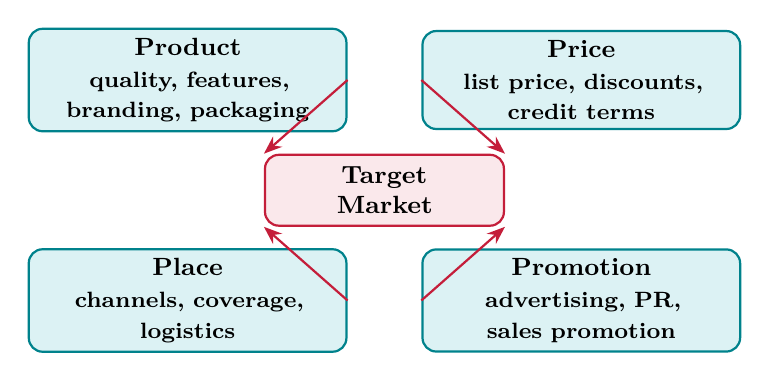
\begin{tikzpicture}[
  pbox/.style={rectangle, draw=myteal, fill=hdrteal, text width=3.8cm,
    align=center, minimum height=1.2cm, font=\small\bfseries,
    rounded corners=5pt, line width=0.8pt},
  tbox/.style={rectangle, draw=myred, fill=hdrred, text width=2.8cm,
    align=center, minimum height=0.9cm, font=\small\bfseries,
    rounded corners=5pt, line width=0.8pt}
]
  % 2x2 grid of P-boxes
  \node[pbox] (prod)  at (-2.5,  1.4) {Product\\[2pt]{\footnotesize quality, features,\\branding, packaging}};
  \node[pbox] (price) at ( 2.5,  1.4) {Price\\[2pt]{\footnotesize list price, discounts,\\credit terms}};
  \node[pbox] (place) at (-2.5, -1.4) {Place\\[2pt]{\footnotesize channels, coverage,\\logistics}};
  \node[pbox] (promo) at ( 2.5, -1.4) {Promotion\\[2pt]{\footnotesize advertising, PR,\\sales promotion}};

  % Central target node
  \node[tbox] (tm) at (0, 0) {\textbf{Target\\Market}};

  % Arrows from each P to target
  \draw[redarrow] (prod.east)  -- (tm.north west);
  \draw[redarrow] (price.west) -- (tm.north east);
  \draw[redarrow] (place.east) -- (tm.south west);
  \draw[redarrow] (promo.west) -- (tm.south east);
\end{tikzpicture}
\end{tcolorbox}

\par\noindent
{\renewcommand{\arraystretch}{1.55}%
\begin{tabularx}{\linewidth}{|B{2.2cm}|Y|Y|}
\hline
\multicolumn{1}{|>{\centering\arraybackslash\color{white}}m{2.2cm}|}{\textbf{Element}} &
\multicolumn{1}{>{\centering\arraybackslash\color{white}}Y|}{\textbf{Key Decisions}} &
\multicolumn{1}{>{\centering\arraybackslash\color{white}}Y|}{\textbf{Examples}} \\[4pt]
\hline
Product & Design, quality, features, variants, packaging, after-sales service. & iPhone with multiple storage options. \\[4pt]
\hline
Price & Pricing strategy (skimming, penetration, competitive), discounts, payment terms. & Introductory low price for market entry. \\[4pt]
\hline
Place & Distribution channels, intermediaries, logistics, coverage (intensive, selective, exclusive). & Direct online sale vs.\ retail chain. \\[4pt]
\hline
Promotion & Advertising, personal selling, public relations, sales promotions, digital marketing. & TV ad campaign + social media promotion. \\[4pt]
\hline
\end{tabularx}
}

\subsection{Advertising and Brand Management}

\begin{tcolorbox}[defbox, title={\textbf{Advertising and Brand Management}}]
\textbf{Advertising} is any paid form of non-personal presentation and promotion of ideas, goods, or services by an identified sponsor through mass media (TV, radio, print, digital).
\par\vspace{3pt}
\textbf{Brand} is a name, term, sign, symbol, or design (or a combination) intended to identify the goods or services of one seller and to differentiate them from competitors.
\par\vspace{3pt}
\textbf{Brand Equity} is the added value a brand name gives to a product beyond its functional benefits.
\end{tcolorbox}

\textbf{Objectives of Advertising (AIDA Model):}
\begin{enumerate}[label=\textbf{\arabic*.}, leftmargin=*, itemsep=2pt, topsep=2pt]
  \item \textbf{Awareness:} Make the target audience aware of the product/brand.
  \item \textbf{Interest:} Generate interest by highlighting features and benefits.
  \item \textbf{Desire:} Create a desire/preference for the brand over competitors.
  \item \textbf{Action:} Motivate the consumer to purchase.
\end{enumerate}

\textbf{Brand building strategies:}
\begin{itemize}[leftmargin=*, itemsep=2pt]
  \item Consistent quality and customer experience across all touchpoints.
  \item Emotional brand associations and storytelling.
  \item Celebrity endorsements and influencer marketing.
  \item Corporate Social Responsibility (CSR) initiatives that enhance brand image.
\end{itemize}

% ===============================================================================
\section{Operations and Technology Management}
% ===============================================================================

\begin{tcolorbox}[defbox, title={\textbf{Operations Management --- Definition}}]
\textbf{Operations Management (OM)} is the administration of business practices aimed at creating the highest level of efficiency possible within an organisation. It is concerned with converting materials and labour into goods and services as efficiently as possible.
\end{tcolorbox}

\subsection{Production and Operations Management}

\textbf{Types of production systems:}
\par\noindent
{\renewcommand{\arraystretch}{1.55}%
\begin{tabularx}{\linewidth}{|B{3.0cm}|Y|Y|}
\hline
\multicolumn{1}{|>{\centering\arraybackslash}m{3.0cm}|}{\textbf{Type}} &
\multicolumn{1}{>{\centering\arraybackslash}Y|}{\textbf{Description}} &
\multicolumn{1}{>{\centering\arraybackslash}Y|}{\textbf{Example}} \\[4pt]
\hline
Job/Project Production & One-off, custom products made individually. & Ship building, construction. \\[4pt]
\hline
Batch Production & Groups of identical items produced together in stages. & Bakeries, pharmaceuticals. \\[4pt]
\hline
Mass/Flow Production & Continuous, standardised production of large volumes on assembly lines. & Car assembly, electronics. \\[4pt]
\hline
Continuous Process & 24/7 uninterrupted flow production. & Oil refinery, chemical plant. \\
\hline
\end{tabularx}
}

\textbf{Key decisions in Production/Operations Management:}
\begin{itemize}[leftmargin=*, itemsep=2pt]
  \item \textbf{Capacity planning:} Determining production capacity needed to meet demand.
  \item \textbf{Facility layout:} Arrangement of machines, workstations, and storage (process layout, product layout, fixed-position layout).
  \item \textbf{Aggregate planning:} Medium-term production scheduling to match supply with forecasted demand.
  \item \textbf{Inventory management:} Deciding optimal stock levels to balance holding costs vs.\ shortage costs.
\end{itemize}

\begin{tcolorbox}[formulabox, title={\textbf{Economic Order Quantity (EOQ)}}]
The EOQ model minimises total inventory cost (holding + ordering):
\begin{equation}
  Q^* = \sqrt{\frac{2DS}{H}}
\end{equation}
Where:
\begin{itemize}[leftmargin=1.5em, itemsep=1pt, topsep=2pt]
  \item[] $Q^*$ = Optimal order quantity (units)
  \item[] $D$ = Annual demand (units/year)
  \item[] $S$ = Ordering cost per order (\$)
  \item[] $H$ = Annual holding/carrying cost per unit
\end{itemize}
\par\vspace{4pt}
Total Annual Cost: $\displaystyle TC = \frac{D}{Q}S + \frac{Q}{2}H$
\end{tcolorbox}

\subsection{Logistics and Supply Chain Management}

\begin{tcolorbox}[defbox, title={\textbf{Supply Chain Management (SCM)}}]
\textbf{Supply Chain Management} is the management of the flow of goods, services, information, and finances from raw material suppliers through manufacturers and distributors to the final end-user. The goal is to maximise customer value while minimising total system cost.
\end{tcolorbox}

\begin{tcolorbox}[tikzbox, title={Basic Supply Chain Flow}]
\centering
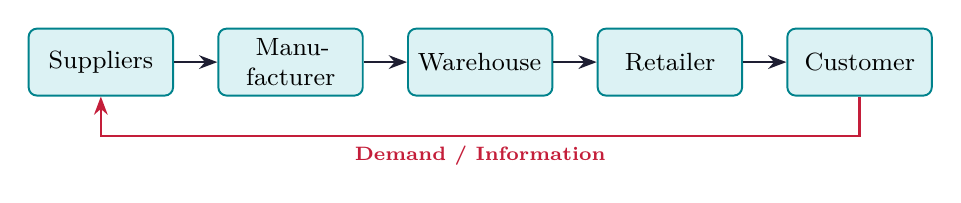
\begin{tikzpicture}[node distance=0.3cm and 0.5cm,
  sblock/.style={rectangle, draw=myteal, fill=hdrteal, text width=1.6cm,
    align=center, minimum height=0.85cm, font=\small, rounded corners=3pt, line width=0.7pt}]
  \node[sblock] (sup) {Suppliers};
  \node[sblock, right=0.55cm of sup] (mfg) {Manufacturer};
  \node[sblock, right=0.55cm of mfg] (wh)  {Warehouse};
  \node[sblock, right=0.55cm of wh]  (ret) {Retailer};
  \node[sblock, right=0.55cm of ret] (cust){Customer};

  \draw[arrow] (sup)--(mfg);
  \draw[arrow] (mfg)--(wh);
  \draw[arrow] (wh)--(ret);
  \draw[arrow] (ret)--(cust);
  \draw[redarrow] (cust.south) -- ++(0,-0.5) -| (sup.south)
    node[pos=0.25, below, font=\scriptsize\bfseries\color{myred}] {Demand / Information};
\end{tikzpicture}
\end{tcolorbox}

\textbf{Key logistics activities:}
\begin{itemize}[leftmargin=*, itemsep=2pt]
  \item Transportation (road, rail, air, sea selection).
  \item Warehousing and inventory storage.
  \item Order processing and fulfilment.
  \item Demand forecasting and supply planning.
  \item Reverse logistics (returns, recycling).
\end{itemize}

\subsection{Total Quality Management (TQM)}

\begin{tcolorbox}[defbox, title={\textbf{Total Quality Management (TQM)}}]
\textbf{TQM} is a management approach centred on quality, based on the participation of all members of an organisation, aimed at long-term success through customer satisfaction and benefits to all members of the organisation and society.
\par\vspace{3pt}
\textbf{Core principle:} Quality is everyone's responsibility, not just the quality control department.
\end{tcolorbox}

\textbf{Key principles of TQM:}
\begin{itemize}[leftmargin=*, itemsep=2pt]
  \item \textbf{Customer Focus:} Understanding and exceeding customer expectations.
  \item \textbf{Continuous Improvement (Kaizen):} Ongoing, incremental improvements in all processes.
  \item \textbf{Employee Involvement:} All employees contribute to quality improvement.
  \item \textbf{Process Approach:} Focus on improving processes to improve outputs.
  \item \textbf{Fact-Based Decision Making:} Use of data and statistical tools.
  \item \textbf{Supplier Relationships:} Mutually beneficial relationships with suppliers.
\end{itemize}

\subsection{Kaizen and Six Sigma}

\begin{tcolorbox}[defbox, title={\textbf{Kaizen and Six Sigma}}]
\textbf{Kaizen} (Japanese: ``change for better'') is a philosophy of continuous, incremental improvement involving everyone in the organisation --- from top management to shop floor workers. It focuses on eliminating waste (Muda) in all forms.
\par\vspace{3pt}
\textbf{Six Sigma} is a data-driven methodology for eliminating defects in any process. The goal is to reduce process variation to achieve no more than \textbf{3.4 defects per million opportunities (DPMO)}.
\end{tcolorbox}

\textbf{Kaizen vs.\ Six Sigma:}
\par\noindent
{\renewcommand{\arraystretch}{1.55}%
\begin{tabularx}{\linewidth}{|B{3.0cm}|Y|Y|}
\hline
\multicolumn{1}{|>{\centering\arraybackslash}m{3.0cm}|}{\textbf{Aspect}} &
\multicolumn{1}{>{\centering\arraybackslash}Y|}{\textbf{Kaizen}} &
\multicolumn{1}{>{\centering\arraybackslash}Y|}{\textbf{Six Sigma}} \\[4pt]
\hline
Origin & Japan (Toyota Production System) & Motorola (1986) \\
\hline
Approach & Incremental, continuous improvement. & Breakthrough improvement; eliminate root causes of defects. \\[4pt]
\hline
Scope & Entire organisation; all processes. & Specific critical processes and projects. \\
\hline
Tools & 5S, PDCA, Value Stream Mapping. & DMAIC, statistical tools (SPC, DOE). \\
\hline
Involvement & All employees (bottom-up). & Trained specialists (Black Belts, Green Belts). \\
\hline
Goal & Reduce waste; improve efficiency. & Reduce variation; achieve near-zero defects. \\
\hline
\end{tabularx}
}

\textbf{The DMAIC Cycle (Six Sigma):}
\begin{enumerate}[label=\textbf{\arabic*.}, leftmargin=*, itemsep=2pt, topsep=2pt]
  \item \textbf{Define:} Define the problem, project scope, customer requirements (CTQs), and project goals.
  \item \textbf{Measure:} Collect baseline data; quantify the current process performance.
  \item \textbf{Analyse:} Identify root causes of defects using statistical tools (Fishbone diagram, Pareto chart, regression).
  \item \textbf{Improve:} Develop, test, and implement solutions to eliminate root causes.
  \item \textbf{Control:} Monitor the improved process to sustain gains using control charts and SOPs.
\end{enumerate}

\textbf{The PDCA Cycle (Kaizen / TQM):}
\begin{enumerate}[label=\textbf{\arabic*.}, leftmargin=*, itemsep=2pt, topsep=2pt]
  \item \textbf{Plan:} Identify a problem; analyse causes; plan improvement.
  \item \textbf{Do:} Implement the planned change on a small scale.
  \item \textbf{Check:} Measure and evaluate results against the plan.
  \item \textbf{Act:} Standardise the improvement if successful; repeat the cycle.
\end{enumerate}

\subsection{Management Information Systems (MIS)}

\begin{tcolorbox}[defbox, title={\textbf{Management Information System (MIS)}}]
\textbf{MIS} is an integrated, user-machine system that provides information to support operations, management, and decision-making functions in an organisation. It collects data from internal and external sources, processes it, and presents it as structured reports and dashboards to managers.
\end{tcolorbox}

\textbf{Types of Information Systems:}
\par\noindent
{\renewcommand{\arraystretch}{1.55}%
\begin{tabularx}{\linewidth}{|B{3.2cm}|Y|Y|}
\hline
\multicolumn{1}{|>{\centering\arraybackslash\color{white}}m{3.2cm}|}{\textbf{System}} &
\multicolumn{1}{>{\centering\arraybackslash\color{white}}Y|}{\textbf{Level}} &
\multicolumn{1}{>{\centering\arraybackslash\color{white}}Y|}{\textbf{Purpose}} \\[4pt]
\hline
TPS (Transaction Processing System) & Operational & Records daily routine transactions (sales, payroll). \\[4pt]
\hline
MIS (Management Information System) & Middle management & Provides structured summary reports for routine decisions. \\[4pt]
\hline
DSS (Decision Support System) & Middle/Top management & Supports semi-structured and unstructured decisions with models. \\[4pt]
\hline
EIS/ESS (Executive Information System) & Top management & Strategic dashboards; external and internal data. \\[4pt]
\hline
ERP (Enterprise Resource Planning) & All levels & Integrates all business functions (finance, HR, supply chain) in a single system. \\[4pt]
\hline
\end{tabularx}
}

\textbf{Benefits of MIS:}
\begin{itemize}[leftmargin=*, itemsep=2pt]
  \item Facilitates faster and more accurate decision-making.
  \item Improves coordination and communication across departments.
  \item Provides real-time monitoring of business performance (KPIs).
  \item Reduces information redundancy and improves data integrity.
\end{itemize}

% ===============================================================================
% MANDATORY QUICK REVISION PAGE
% ===============================================================================
\newpage
\begin{center}
  {\large\bfseries\color{myred} Quick Revision --- Module 4}\\[3pt]
  {\small\color{mydark} Customer Management, Operations, TQM, Kaizen, Six Sigma \& MIS $|$ HS-HU701}
\end{center}
\noindent{\color{myred}\rule{\linewidth}{1.2pt}}
\vspace{4pt}

\begin{tcolorbox}[formulabox, title={\textbf{Key Formulas and Frameworks at a Glance}}]
\renewcommand{\arraystretch}{1.3}
\begin{tabularx}{\linewidth}{B{4.2cm} X}
EOQ & $Q^* = \sqrt{2DS/H}$ \\[4pt]
Total Inventory Cost & $TC = (D/Q)S + (Q/2)H$ \\[4pt]
4Ps of Marketing & Product, Price, Place, Promotion \\[3pt]
AIDA Model & Awareness $\to$ Interest $\to$ Desire $\to$ Action \\[3pt]
DMAIC (Six Sigma) & Define $\to$ Measure $\to$ Analyse $\to$ Improve $\to$ Control \\[3pt]
PDCA (Kaizen/TQM) & Plan $\to$ Do $\to$ Check $\to$ Act \\[3pt]
Six Sigma Target & $\leq$ 3.4 Defects Per Million Opportunities (DPMO) \\
\end{tabularx}
\end{tcolorbox}

\begin{tcolorbox}[defbox, title={\textbf{One-Line Definitions}}]
\begin{itemize}[leftmargin=*, itemsep=2pt, topsep=0pt]
  \item \textbf{Marketing Mix (4Ps):} Controllable tools (Product, Price, Place, Promotion) blended to target a market.
  \item \textbf{Brand Equity:} Extra value a brand name adds to a product beyond its functional benefits.
  \item \textbf{Operations Management:} Converting inputs (materials, labour) into goods/services as efficiently as possible.
  \item \textbf{EOQ:} Order quantity that minimises the sum of annual ordering cost and holding cost.
  \item \textbf{Supply Chain Management:} Managing the flow of goods and information from supplier to end customer.
  \item \textbf{TQM:} Organisation-wide approach to embedding quality in all processes to achieve customer satisfaction.
  \item \textbf{Kaizen:} Continuous, incremental improvement involving all employees to eliminate waste.
  \item \textbf{Six Sigma:} Data-driven methodology targeting $\leq$ 3.4 DPMO through root cause elimination.
  \item \textbf{DMAIC:} Six Sigma improvement cycle: Define, Measure, Analyse, Improve, Control.
  \item \textbf{MIS:} Integrated system that provides managers with information for decision-making.
  \item \textbf{ERP:} Software that integrates all core business processes into a single unified system.
\end{itemize}
\end{tcolorbox}

\begin{tcolorbox}[exambox, title={\textbf{Frequently Asked / Viva Questions}}]
\begin{enumerate}[topsep=0pt, label=\textbf{Q\arabic*.}, itemsep=5pt]
  \item \Q{What are the 4Ps of the Marketing Mix? Give one example for each.}
    Product (iPhone), Price (penetration pricing), Place (online store), Promotion (TV advertisement).
  \item \Q{What is the AIDA model in advertising?}
    AIDA stands for Awareness (make customers aware), Interest (highlight benefits), Desire (create preference), Action (prompt purchase). It describes the stages a consumer goes through from first exposure to buying.
  \item \Q{What is brand equity and why is it important?}
    Brand equity is the added value a brand name confers to a product. It is important because it enables premium pricing, customer loyalty, and competitive advantage (e.g., Apple vs.\ a generic smartphone).
  \item \Q{Define Supply Chain Management. Draw a simple supply chain.}
    SCM manages the flow of goods, services, and information from raw material suppliers to the final customer. Flow: Suppliers $\to$ Manufacturer $\to$ Warehouse $\to$ Retailer $\to$ Customer (with information flowing back).
  \item \Q{State the EOQ formula and define each variable.}
    $Q^* = \sqrt{2DS/H}$. $D$ = annual demand, $S$ = cost per order, $H$ = annual holding cost per unit. It gives the order quantity that minimises total annual inventory cost.
  \item \Q{What is TQM? What are its core principles?}
    TQM is an organisation-wide philosophy to embed quality in all processes for long-term customer satisfaction. Core principles: customer focus, continuous improvement, employee involvement, process approach, data-based decisions, and supplier relationships.
  \item \Q{What is Kaizen? How does it differ from Six Sigma?}
    Kaizen is continuous, incremental improvement through small daily changes involving all employees (bottom-up). Six Sigma is a project-based breakthrough methodology using statistical tools to reduce defects to 3.4 DPMO (specialist-driven).
  \item \Q{Explain the DMAIC cycle used in Six Sigma.}
    Define (problem and CTQs) $\to$ Measure (baseline performance) $\to$ Analyse (root causes) $\to$ Improve (implement solutions) $\to$ Control (sustain gains with control charts and SOPs).
  \item \Q{What is a Management Information System (MIS)?}
    MIS is an integrated system that collects, processes, and presents data as structured reports to support managerial decision-making at middle levels of the organisation.
  \item \Q{How does an ERP system differ from an MIS?}
    MIS provides reports for management decisions; ERP integrates all business functions (finance, HR, production, supply chain) across the entire organisation into one unified database and application.
  \item \Q{What is the PDCA cycle? Where is it used?}
    PDCA (Plan--Do--Check--Act) is a four-step iterative quality improvement cycle. Used in TQM and Kaizen to continuously improve processes, products, and services.
  \item \Q{What is the difference between intensive, selective, and exclusive distribution?}
    Intensive distribution places products in as many outlets as possible (e.g., soft drinks). Selective distribution uses a limited number of chosen outlets (e.g., electronics). Exclusive distribution uses a single outlet per region (e.g., luxury cars, high-end watches).
\end{enumerate}
\end{tcolorbox}

\begin{tcolorbox}[tikzbox, title={TQM vs.\ Kaizen vs.\ Six Sigma --- Quick Reference}]
\centering
\renewcommand{\arraystretch}{1.4}
{\renewcommand{\arraystretch}{1.55}%
\begin{tabularx}{\linewidth}{|B{2.5cm}|Y|Y|Y|}
\hline
\multicolumn{1}{|>{\centering\arraybackslash}m{2.5cm}|}{\textbf{Aspect}} &
\multicolumn{1}{>{\centering\arraybackslash}Y|}{\textbf{TQM}} &
\multicolumn{1}{>{\centering\arraybackslash}Y|}{\textbf{Kaizen}} &
\multicolumn{1}{>{\centering\arraybackslash}Y|}{\textbf{Six Sigma}} \\[4pt]
\hline
Focus & Overall quality culture & Continuous small improvements & Eliminate defect root causes \\
\hline
Approach & Cultural/philosophical & Incremental (bottom-up) & Statistical/project-based \\
\hline
Cycle & PDCA & PDCA & DMAIC \\
\hline
People & Everyone & Everyone & Black/Green Belts \\
\hline
Target & Customer satisfaction & Waste elimination & $\leq$ 3.4 DPMO \\
\hline
\end{tabularx}
}
\end{tcolorbox}

\end{document}
